\chapter{Input Data}

In some configurations, \glc\ requires additional input data to run. For example, if asked to process galaxy formation through a set of externally derived merger trees, then a file describing those trees must be given. In the remainder of this section we describe the structure of external datasets which can be inputs to \glc.

\section{Broadband Filters}\index{filters!broadband}

To compute luminosities through a given filter, \glc\ requires the response function, $R(\lambda)$, of that filter to be defined. \glc\ follows the convention of \cite{hogg_k_2002} in defining the filter response to be the fraction of incident photons received by the detector at a given wavelength, multiplied by the relative photon response (which will be 1 for a photon-counting detector such as a CCD, or proportional to the photon energy for a bolometer/calorimeter type detector. Filter response files are stored in {\normalfont \ttfamily data/filters/}. Their structure is shown below, with the {\normalfont \ttfamily SDSS\_g.xml} filter reponse file used as an example:
\begin{verbatim}
 <filter>
  <description>SDSS g vacuum (filter+CCD +0 air mass)</description>
  <name>SDSS g</name>
  <origin>Michael Blanton</origin>
  <response>
    <datum>   3630.000      0.0000000E+00</datum>
    <datum>   3680.000      2.2690000E-03</datum>
    <datum>   3730.000      5.4120002E-03</datum>
    <datum>   3780.000      9.8719997E-03</datum>
    <datum>   3830.000      2.9449999E-02</datum>
    .
    .
    . 
  </response>
  <effectiveWavelength>4727.02994472695</effectiveWavelength>
  <vegaOffset>0.107430167298754</vegaOffset>
</filter>
\end{verbatim}
The {\normalfont \ttfamily description} tag should provide a description of the filter, while the {\normalfont \ttfamily name} tag provides a shorter name. The {\normalfont \ttfamily origin} tag should describe from where/whom this filter originated. The {\normalfont \ttfamily response} element contains a list of {\normalfont \ttfamily datum} tags each giving a wavelength (in Angstroms) and response pair. The normalization of the response is arbitrary. The {\normalfont \ttfamily effectiveWavelength} tag gives the mean, response-weighted wavelength of the filter and is used, for example, in dust attenuation calculations. The {\normalfont \ttfamily vegaOffset} tag gives the value (in magnitudes) which must be added to an AB-system magnitude in this system to place it into the Vega system. Both {\normalfont \ttfamily effectiveWavelength} and {\normalfont \ttfamily vegaOffset} can be computed by running
\begin{verbatim}
 scripts/filters/vega_offset_effective_lambda.pl data/filters
\end{verbatim}
which will compute these values for any filter files that do not already contain them and append them to the files.

\section{Merger Trees}\label{sec:MergerTreeFiles}

While \glc\ can build merger trees using analytic methods it is often useful to be able to utilize merger trees from other sources (e.g. extracted from an N-body simulation). To facilitate this, \glc\ allows merger trees to be read from an HDF5 file\footnote{The following assumes that merger trees will be read from a file following \protect\glc's standard HDF5 format which is described in \S\protect\ref{sec:MergerTreeFileFormat}. Other formats can also be read by selecting the relevant importer via the {\normalfont \ttfamily [mergerTreeImporterMethod]} parameter.}. To do so, set the {\normalfont \ttfamily [mergerTreeConstructMethod]} input parameter to {\normalfont \ttfamily read} and specify the filename to read via their {\normalfont \ttfamily [mergerTreeReadFileName]} parameter.

The HDF5 file should follow the general purpose format described in \S\ref{sec:MergerTreeFileFormat}. An example of how to construct such a file can be found in the {\normalfont \ttfamily tests/nBodyMergerTrees} folder. In that folder, the {\normalfont \ttfamily getMillenniumTrees.pl} script will retrieve a sample of merger trees from the \href{http://www.g-vo.org/MyMillennium3/}{Millennium Simulation database} and use the {\normalfont \ttfamily Merger\_Tree\_File\_Maker.exe} code supplied with \glc\ to convert these into an HDF5 file suitable for reading into \glc. The {\normalfont \ttfamily getMillenniumTrees.pl} script requires you to have a username and password to access the Millennium Simulation database\footnote{If you do not have a username and password for the Millennium Simulation database you can request one from \href{mailto:contact@g-vo.org}{\normalfont \ttfamily contact@g-vo.org}.}. These can be entered manually or stored in a section of the {\normalfont \ttfamily galacticusConfig.xml} file (see \S\ref{sec:ConfigFile}) as follows:
\begin{verbatim}
  <millenniumDB>
    <host>
      <name>^myHost$</name>
      <user>myUserName</user>
      <passwordFrom>input</passwordFrom>
      <treePath>/path/to/trees</treePath>
    </host>
    <host>
      <name>default</name>
      <user>myUserName</user>
      <password>myPassword</password>
    </host>
  </millenniumDB>
\end{verbatim}
Here, each {\normalfont \ttfamily host} section describes rules for a given computer (with ``default'' being used if no specific match to the regular expression give in {\normalfont \ttfamily name} is found). The {\normalfont \ttfamily user} element gives the user name to use, while the {\normalfont \ttfamily passwordFrom} element specifies how the password should be obtained. Currently the only allowed mechanism is ``input'', in which case the password is read from standard input. Alternatively, you can include a {\normalfont \ttfamily password} element which contains the password itself. Of course, this is insecure\ldots

The optional {\normalfont \ttfamily treePath} element gives the location where merger trees from the Millennium Simulation can be stored. Some scripts will make use of this location so that Millennium Simulation merger trees can be shared between multiple scripts.

\subsection{Processing of Merger Tree Files}\label{sec:MergerTreeFileProcessing}

The ``read'' merger tree construction method (see \S\ref{sec:MergerTreeConstruction}) reads these files and processes them into a form suitable for \glc\ to evolve. Merger trees are inherently complex structures, particularly when the possibility of subhalos are considered. \glc\ is currently designed to work with single descendent merger trees, i.e. ones in which the tree structure is entirely defined by specifying which \gls{node} a given \gls{node} is physically associated with at a later time. Additionally, \glc\ expects the merger tree file to contain information on the host \gls{node}, i.e. the node within which a given node is physically located. In the following, these two properties are labelled {\normalfont \ttfamily descendentNode} and {\normalfont \ttfamily hostNode}. \glc\ assumes that nodes for which {\normalfont \ttfamily descendentNode}$=${\normalfont \ttfamily hostNode} are isolated halos (i.e. they are their own hosts) while other nodes are subhalos (i.e. they are hosted by some other node). An example of a simple tree structure is shown in Fig.~\ref{fig:MergerTreeSimple}. The particular structure would be represented by the following list of nodes and node properties (a $-1$ indicates that no descendent node exists):
\begin{center}
\begin{tabular}{rrr}
\hline
{\normalfont \ttfamily node} & {\normalfont \ttfamily descendentNode} & {\normalfont \ttfamily hostNode} \\
\hline
1 & -1 & 1 \\
2 &  1 & 2 \\
3 &  2 & 3 \\
4 &  1 & 4 \\
5 &  4 & 5 \\
6 & -1 & 1 \\
7 &  6 & 4 \\
8 &  7 & 8 \\
\hline
\end{tabular}
\end{center}

\begin{figure}
 \begin{center}
 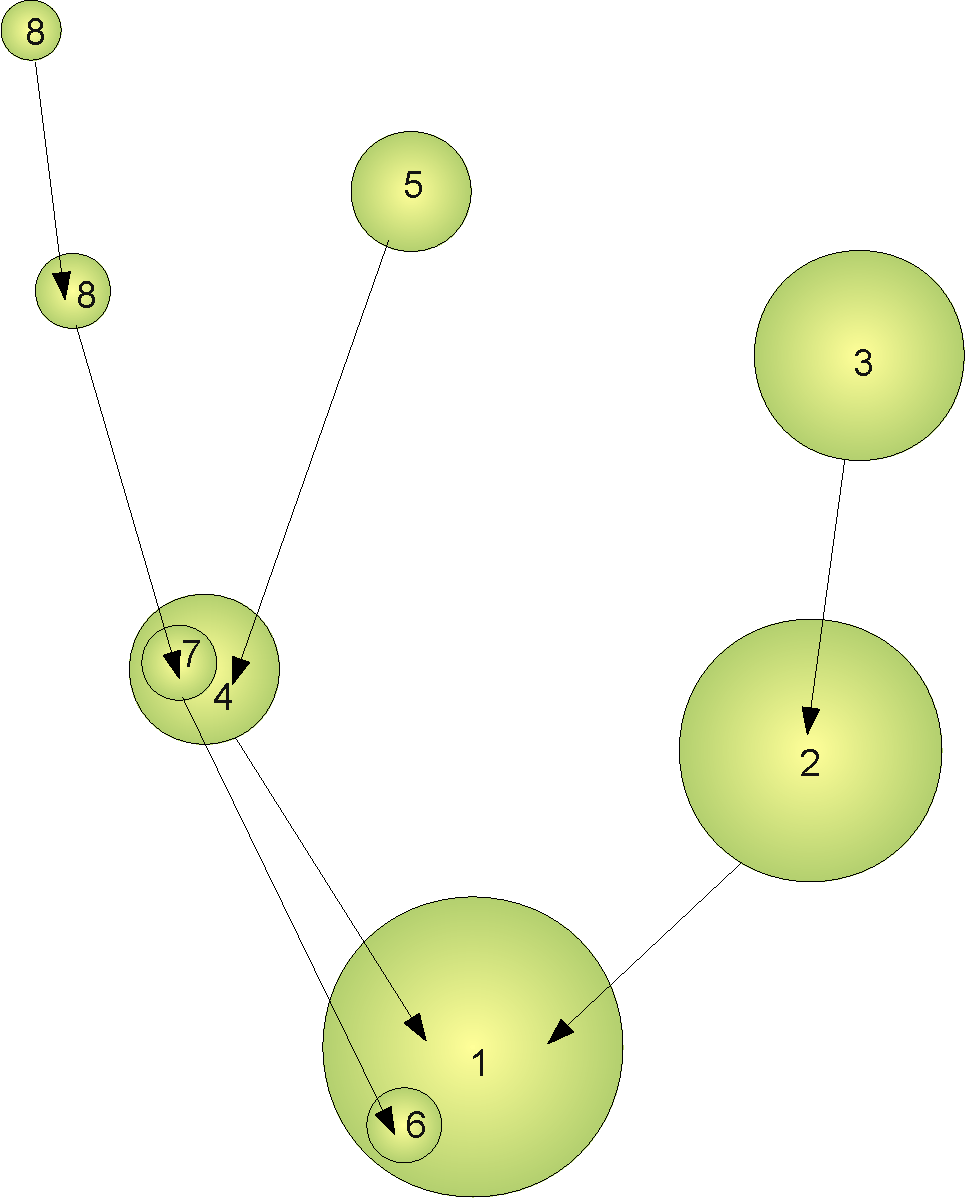
\includegraphics[width=160mm]{Diagrams/MergerTreeSimple.pdf}
 \end{center}
 \caption{An example of a simple merger tree structure. Colored circles represent nodes in the merger tree. Each node has a unique index indicated by the number inside each circle. Black arrows link each node to its descendent node (as specified by the {\normalfont \ttfamily descendentNode} property. Where a node is not its own host node it is placed inside its host node.}
 \label{fig:MergerTreeSimple}
\end{figure}

The following should be noted when constructing merger tree files:
\begin{itemize}
\item Note that \glc\ does not require that nodes be placed on a uniform grid of times/redshifts, nor that mass be conserved along a branch of the tree. After processing the tree in this way, \glc\ builds additional links which identify the child node of each halo and any sibling nodes. These are not required to specify the tree structure but are computationally convenient.
\item It is acceptable for a node to begin its existence as a subhalo (i.e. to have never had an isolated node progenitor). Such nodes will be created as satellites in the merger tree and, providing the selected node components (see \S\ref{sec:Components}) initialize their properties appropriately, will be evolved correctly.
\item It is acceptable for an isolated node to have progenitors, none of which are a primary progenitor. This can happen if all progenitors descend into subhalos in the isolated node. In such cases, \glc\ will create a clone of the isolated node at a very slightly earlier time to act as the primary progenitor. This is necessary to allow the tree to be processed correctly, but does not affect the evolution of the tree.
\item Normally, cases where a node's host node cannot be found in the \gls{forest} will cause \glc\ to exit with an error. Setting {\normalfont \ttfamily [mergerTreeReadMissingHostsAreFatal]}$=${\normalfont \ttfamily false} will instead circumvent this issue by making any such nodes self-hosting (i.e. they become isolated nodes rather than subhalos). Note that this behavior is not a physically correct way to treat such cases---it is intended only to allow trees to be processed in cases where the full \gls{forest} is not available.
\item It is acceptable for nodes to jump between branches in a tree, or even to jump between branches in different trees. In the latter case, all trees linked by jumping nodes (a so-called ``\gls{forest}'' of connected trees) must be stored as a single forest (with multiple root-nodes) in the merger tree file. \glc\ will process this \gls{forest} of trees simultaneously, allowing to nodes to move between their branches.
\item It is acceptable for a subhalo to later become an isolated halo (as can happen due to three-body interactions; see  \citealt{sales_cosmic_2007}). If {\normalfont \ttfamily [mergerTreeReadAllowSubhaloPromotions]}$=${\normalfont \ttfamily true} then such cases will be handled correctly (i.e. the subhalo will be promoted back to being an isolated halo). If {\normalfont \ttfamily [mergerTreeReadAllowSubhaloPromotions]}$=${\normalfont \ttfamily false} then subhalos are not permitted to become isolated halos. In this case, the following logic will be applied to remove all such cases from the tree:\\

\noindent\hspace{ 5mm} $\rightarrow$ \parbox[t]{150mm}{For any branch in a tree which at some point is a subhalo:}\\

\noindent\hspace{10mm} $\rightarrow$ \parbox[t]{145mm}{Beginning from the earliest node in the branch that is a subhalo, repeatedly step to the next descendent node;}\\

\noindent\hspace{10mm} $\rightarrow$ \parbox[t]{145mm}{If that descendent is \emph{not} a subhalo then:}\\

\noindent\hspace{15mm} $\rightarrow$ \parbox[t]{140mm}{If there is not currently any non-subhalo node which has the present node as its descendent then current node is only descendent of a subhalo. Therefore, try to make this node a subhalo, and propose the descendent of the host node of the previous node visited in the branch as the new host:}\\

\noindent\hspace{20mm} $\rightarrow$ \parbox[t]{135mm}{If the proposed host exists:}\\

\noindent\hspace{25mm} $\rightarrow$ \parbox[t]{130mm}{If the mass of the current node is less than that of the proposed host:}\\

\noindent\hspace{30mm} $\rightarrow$ \parbox[t]{125mm}{If the proposed hosts exists before the current node, repeatedly step to its descendents until one is found which exists at or after the time of the current node. This is the new proposed host.}\\

\noindent\hspace{30mm} $\rightarrow$ \parbox[t]{125mm}{If the proposed host is a subhalo, make it an isolated node.}\\

\noindent\hspace{30mm} $\rightarrow$ \parbox[t]{125mm}{The current node is made a subhalo within the proposed host.}\\

\noindent\hspace{25mm} $\rightarrow$ \parbox[t]{130mm}{Otherwise:}\\

\noindent\hspace{30mm} $\rightarrow$ \parbox[t]{125mm}{The current node remains an isolated node, while the proposed host is instead made a subhalo within the current node.}\\

\noindent\hspace{20mm} $\rightarrow$ \parbox[t]{135mm}{Otherwise:}\\

\noindent\hspace{25mm} $\rightarrow$ \parbox[t]{130mm}{The proposed host does not exists, which implies the end of a branch has been reached. Therefore, flag the current node as being a subhalo with a host identical to that of the node from which it descended.}\\
\end{itemize}

\subsubsection{Requirements for \glc\ Input Parameters}

The following requirements must be met for the input parameters to \glc\ when using merger trees read from file:
\begin{itemize}
 \item The cosmological parameters ($\Omega_{\mathrm M}$, $\Omega_\Lambda$, $\Omega_{\mathrm b}$, $H_0$, $\sigma_8$), if defined in the file, must be set identically in the \glc\ input file unless you set {\normalfont \ttfamily [mergerTreeReadMismatchIsFatal]}$=${\normalfont \ttfamily false} in which case you'll just be warned about any mismatch;
 \item \glc\ assumes by default that all merger trees exist at the final output time---if this is not the case set {\normalfont \ttfamily [allTreesExistAtFinalTime]}$=${\normalfont \ttfamily false}.
\end{itemize}

\subsection{Setting of Halo Properties}

\subsubsection{Dark Matter Scale Radii}\index{dark matter halo!concentration}\index{dark matter halo!scale radius}

If {\normalfont \ttfamily [mergerTreeReadPresetScaleRadii]}$=${\normalfont \ttfamily true} and the {\normalfont \ttfamily halfMassRadius} dataset is available within the {\normalfont \ttfamily haloTrees} group (see \S\ref{sec:ForestHalosGroup}) then the half-mass radii of nodes will be used to compute the corresponding scale length of the dark matter halo profile\footnote{The scale radius is found by seeking a value which gives the correct half mass radius. It is therefore important that the definition of halo mass (specifically the virial overdensity) in \protect\glc\ be the same as was used in computing the input half mass radii.}. This requires a dark matter profile scale component which supports setting of the scale length (see \S\ref{sec:DarkMatterProfileComponent}).

\subsubsection{Satellite Merger Times}\index{merger times}\index{satellite!merger times}

If {\normalfont \ttfamily [mergerTreeReadPresetMergerTimes]}$=${\normalfont \ttfamily true} then merger times for satellites will be computed directly from the merger tree data read from file. When a subhalo has an isolated halo as a descendent it is assumed to undergo a merger with that isolated halo at that time. Note that this requires a satellite orbit component method which supports setting of merger times (e.g. {\normalfont \ttfamily [treeNodeMethodSatelliteOrbit]}$=${\normalfont \ttfamily preset}).

\subsubsection{Dark Matter Halo Spins}\index{dark matter halo!spin}

If {\normalfont \ttfamily [mergerTreeReadPresetSpins]}$=${\normalfont \ttfamily true} and the {\normalfont \ttfamily angularMomentum} dataset is available within the {\normalfont \ttfamily haloTrees} group (see \S\ref{sec:ForestHalosGroup}) then the spin parameters of nodes will be computed and set. This requires a dark matter halo spin component which supports setting of the spin (see \S\ref{sec:DarkMatterHaloSpinComponent}).
